%-*-latex-*-
\sectionthree{\cpp\ STL deque: \texttt{std::deque}}
\begin{python0}
from solutions import *; clear()
\end{python0}

The \cpp\ STL \verb!std::deque! (double ended queue) class is a double-ended
queue but the implementation usually uses dynamic arrays, i.e.,
it's not implemented using a doubly-linked list.
Specifically, \verb!std::deque! is implemented as a
vector of pointers to
vectors of the same size.

Run and study the following very carefully:
\VerbatimInput[frame=single,fontsize=\footnotesize]{deque/main.cpp}
Here's the output:
\begin{center}
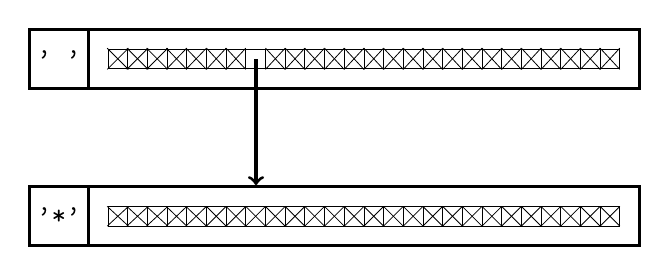
\begin{tikzpicture}

\draw (0.125, 0.125)
  node[draw, line width=0.01cm, , color=black,
       rounded corners=0cm, inner sep=0cm] {

\begin{minipage}[t][0.25cm]{0.25cm}
\mbox{}

\end{minipage}

};
\draw (0.375, 0.125)
  node[draw, line width=0.01cm, , color=black,
       rounded corners=0cm, inner sep=0cm] {

\begin{minipage}[t][0.25cm]{0.25cm}
\mbox{}

\end{minipage}

};
\draw (0.625, 0.125)
  node[draw, line width=0.01cm, , color=black,
       rounded corners=0cm, inner sep=0cm] {

\begin{minipage}[t][0.25cm]{0.25cm}
\mbox{}

\end{minipage}

};
\draw (0.875, 0.125)
  node[draw, line width=0.01cm, , color=black,
       rounded corners=0cm, inner sep=0cm] {

\begin{minipage}[t][0.25cm]{0.25cm}
\mbox{}

\end{minipage}

};
\draw (1.125, 0.125)
  node[draw, line width=0.01cm, , color=black,
       rounded corners=0cm, inner sep=0cm] {

\begin{minipage}[t][0.25cm]{0.25cm}
\mbox{}

\end{minipage}

};
\draw (1.375, 0.125)
  node[draw, line width=0.01cm, , color=black,
       rounded corners=0cm, inner sep=0cm] {

\begin{minipage}[t][0.25cm]{0.25cm}
\mbox{}

\end{minipage}

};
\draw (1.625, 0.125)
  node[draw, line width=0.01cm, , color=black,
       rounded corners=0cm, inner sep=0cm] {

\begin{minipage}[t][0.25cm]{0.25cm}
\mbox{}

\end{minipage}

};
\draw (1.875, 0.125)
  node[draw, line width=0.01cm, , color=black,
       rounded corners=0cm, inner sep=0cm] {

\begin{minipage}[t][0.25cm]{0.25cm}
\mbox{}

\end{minipage}

};
\draw (2.125, 0.125)
  node[draw, line width=0.01cm, , color=black,
       rounded corners=0cm, inner sep=0cm] {

\begin{minipage}[t][0.25cm]{0.25cm}
\mbox{}

\end{minipage}

};
\draw (2.375, 0.125)
  node[draw, line width=0.01cm, , color=black,
       rounded corners=0cm, inner sep=0cm] {

\begin{minipage}[t][0.25cm]{0.25cm}
\mbox{}

\end{minipage}

};
\draw (2.625, 0.125)
  node[draw, line width=0.01cm, , color=black,
       rounded corners=0cm, inner sep=0cm] {

\begin{minipage}[t][0.25cm]{0.25cm}
\mbox{}

\end{minipage}

};
\draw (2.875, 0.125)
  node[draw, line width=0.01cm, , color=black,
       rounded corners=0cm, inner sep=0cm] {

\begin{minipage}[t][0.25cm]{0.25cm}
\mbox{}

\end{minipage}

};
\draw (3.125, 0.125)
  node[draw, line width=0.01cm, , color=black,
       rounded corners=0cm, inner sep=0cm] {

\begin{minipage}[t][0.25cm]{0.25cm}
\mbox{}

\end{minipage}

};
\draw (3.375, 0.125)
  node[draw, line width=0.01cm, , color=black,
       rounded corners=0cm, inner sep=0cm] {

\begin{minipage}[t][0.25cm]{0.25cm}
\mbox{}

\end{minipage}

};
\draw (3.625, 0.125)
  node[draw, line width=0.01cm, , color=black,
       rounded corners=0cm, inner sep=0cm] {

\begin{minipage}[t][0.25cm]{0.25cm}
\mbox{}

\end{minipage}

};
\draw (3.875, 0.125)
  node[draw, line width=0.01cm, , color=black,
       rounded corners=0cm, inner sep=0cm] {

\begin{minipage}[t][0.25cm]{0.25cm}
\mbox{}

\end{minipage}

};
\draw (4.125, 0.125)
  node[draw, line width=0.01cm, , color=black,
       rounded corners=0cm, inner sep=0cm] {

\begin{minipage}[t][0.25cm]{0.25cm}
\mbox{}

\end{minipage}

};
\draw (4.375, 0.125)
  node[draw, line width=0.01cm, , color=black,
       rounded corners=0cm, inner sep=0cm] {

\begin{minipage}[t][0.25cm]{0.25cm}
\mbox{}

\end{minipage}

};
\draw (4.625, 0.125)
  node[draw, line width=0.01cm, , color=black,
       rounded corners=0cm, inner sep=0cm] {

\begin{minipage}[t][0.25cm]{0.25cm}
\mbox{}

\end{minipage}

};
\draw (4.875, 0.125)
  node[draw, line width=0.01cm, , color=black,
       rounded corners=0cm, inner sep=0cm] {

\begin{minipage}[t][0.25cm]{0.25cm}
\mbox{}

\end{minipage}

};
\draw (5.125, 0.125)
  node[draw, line width=0.01cm, , color=black,
       rounded corners=0cm, inner sep=0cm] {

\begin{minipage}[t][0.25cm]{0.25cm}
\mbox{}

\end{minipage}

};
\draw (5.375, 0.125)
  node[draw, line width=0.01cm, , color=black,
       rounded corners=0cm, inner sep=0cm] {

\begin{minipage}[t][0.25cm]{0.25cm}
\mbox{}

\end{minipage}

};
\draw (5.625, 0.125)
  node[draw, line width=0.01cm, , color=black,
       rounded corners=0cm, inner sep=0cm] {

\begin{minipage}[t][0.25cm]{0.25cm}
\mbox{}

\end{minipage}

};
\draw (5.875, 0.125)
  node[draw, line width=0.01cm, , color=black,
       rounded corners=0cm, inner sep=0cm] {

\begin{minipage}[t][0.25cm]{0.25cm}
\mbox{}

\end{minipage}

};
\draw (6.125, 0.125)
  node[draw, line width=0.01cm, , color=black,
       rounded corners=0cm, inner sep=0cm] {

\begin{minipage}[t][0.25cm]{0.25cm}
\mbox{}

\end{minipage}

};
\draw (6.375, 0.125)
  node[draw, line width=0.01cm, , color=black,
       rounded corners=0cm, inner sep=0cm] {

\begin{minipage}[t][0.25cm]{0.25cm}
\mbox{}

\end{minipage}

};
\draw (3.25, 0.125)
  node[draw, line width=0.04cm, , color=black,
       rounded corners=0cm, inner sep=0cm] {

\begin{minipage}[t][0.75cm]{7.0cm}
\mbox{}

\end{minipage}

};\draw[line width=0.01cm,black] (-0.01,0.26) to  (0.26,-0.01);
\draw[line width=0.01cm,black] (0.26,0.26) to  (-0.01,-0.01);
\draw[line width=0.01cm,black] (0.24,0.26) to  (0.51,-0.01);
\draw[line width=0.01cm,black] (0.51,0.26) to  (0.24,-0.01);
\draw[line width=0.01cm,black] (0.49,0.26) to  (0.76,-0.01);
\draw[line width=0.01cm,black] (0.76,0.26) to  (0.49,-0.01);
\draw[line width=0.01cm,black] (0.74,0.26) to  (1.0,-0.01);
\draw[line width=0.01cm,black] (1.0,0.26) to  (0.74,-0.01);
\draw[line width=0.01cm,black] (0.99,0.26) to  (1.25,-0.01);
\draw[line width=0.01cm,black] (1.25,0.26) to  (0.99,-0.01);
\draw[line width=0.01cm,black] (1.25,0.26) to  (1.5,-0.01);
\draw[line width=0.01cm,black] (1.5,0.26) to  (1.25,-0.01);
\draw[line width=0.01cm,black] (1.5,0.26) to  (1.75,-0.01);
\draw[line width=0.01cm,black] (1.75,0.26) to  (1.5,-0.01);
\draw[line width=0.01cm,black] (2.0,0.26) to  (2.25,-0.01);
\draw[line width=0.01cm,black] (2.25,0.26) to  (2.0,-0.01);
\draw[line width=0.01cm,black] (2.25,0.26) to  (2.5,-0.01);
\draw[line width=0.01cm,black] (2.5,0.26) to  (2.25,-0.01);
\draw[line width=0.01cm,black] (2.5,0.26) to  (2.75,-0.01);
\draw[line width=0.01cm,black] (2.75,0.26) to  (2.5,-0.01);
\draw[line width=0.01cm,black] (2.75,0.26) to  (3.0,-0.01);
\draw[line width=0.01cm,black] (3.0,0.26) to  (2.75,-0.01);
\draw[line width=0.01cm,black] (3.0,0.26) to  (3.25,-0.01);
\draw[line width=0.01cm,black] (3.25,0.26) to  (3.0,-0.01);
\draw[line width=0.01cm,black] (3.25,0.26) to  (3.5,-0.01);
\draw[line width=0.01cm,black] (3.5,0.26) to  (3.25,-0.01);
\draw[line width=0.01cm,black] (3.5,0.26) to  (3.75,-0.01);
\draw[line width=0.01cm,black] (3.75,0.26) to  (3.5,-0.01);
\draw[line width=0.01cm,black] (3.75,0.26) to  (4.0,-0.01);
\draw[line width=0.01cm,black] (4.0,0.26) to  (3.75,-0.01);
\draw[line width=0.01cm,black] (4.0,0.26) to  (4.25,-0.01);
\draw[line width=0.01cm,black] (4.25,0.26) to  (4.0,-0.01);
\draw[line width=0.01cm,black] (4.25,0.26) to  (4.5,-0.01);
\draw[line width=0.01cm,black] (4.5,0.26) to  (4.25,-0.01);
\draw[line width=0.01cm,black] (4.5,0.26) to  (4.75,-0.01);
\draw[line width=0.01cm,black] (4.75,0.26) to  (4.5,-0.01);
\draw[line width=0.01cm,black] (4.75,0.26) to  (5.0,-0.01);
\draw[line width=0.01cm,black] (5.0,0.26) to  (4.75,-0.01);
\draw[line width=0.01cm,black] (5.0,0.26) to  (5.25,-0.01);
\draw[line width=0.01cm,black] (5.25,0.26) to  (5.0,-0.01);
\draw[line width=0.01cm,black] (5.25,0.26) to  (5.5,-0.01);
\draw[line width=0.01cm,black] (5.5,0.26) to  (5.25,-0.01);
\draw[line width=0.01cm,black] (5.5,0.26) to  (5.75,-0.01);
\draw[line width=0.01cm,black] (5.75,0.26) to  (5.5,-0.01);
\draw[line width=0.01cm,black] (5.75,0.26) to  (6.0,-0.01);
\draw[line width=0.01cm,black] (6.0,0.26) to  (5.75,-0.01);
\draw[line width=0.01cm,black] (6.0,0.26) to  (6.25,-0.01);
\draw[line width=0.01cm,black] (6.25,0.26) to  (6.0,-0.01);
\draw[line width=0.01cm,black] (6.25,0.26) to  (6.5,-0.01);
\draw[line width=0.01cm,black] (6.5,0.26) to  (6.25,-0.01);

\draw (-0.625, 0.125)
  node[draw, line width=0.04cm, , color=black,
       rounded corners=0cm, inner sep=0cm] {

\begin{minipage}[t][0.75cm]{0.75cm}
\mbox{}

\end{minipage}

};\draw (-0.625, 0.125) node[color=black] {\texttt{' '}};
\draw (0.125, -1.875)
  node[draw, line width=0.01cm, , color=black,
       rounded corners=0cm, inner sep=0cm] {

\begin{minipage}[t][0.25cm]{0.25cm}
\mbox{}

\end{minipage}

};
\draw (0.375, -1.875)
  node[draw, line width=0.01cm, , color=black,
       rounded corners=0cm, inner sep=0cm] {

\begin{minipage}[t][0.25cm]{0.25cm}
\mbox{}

\end{minipage}

};
\draw (0.625, -1.875)
  node[draw, line width=0.01cm, , color=black,
       rounded corners=0cm, inner sep=0cm] {

\begin{minipage}[t][0.25cm]{0.25cm}
\mbox{}

\end{minipage}

};
\draw (0.875, -1.875)
  node[draw, line width=0.01cm, , color=black,
       rounded corners=0cm, inner sep=0cm] {

\begin{minipage}[t][0.25cm]{0.25cm}
\mbox{}

\end{minipage}

};
\draw (1.125, -1.875)
  node[draw, line width=0.01cm, , color=black,
       rounded corners=0cm, inner sep=0cm] {

\begin{minipage}[t][0.25cm]{0.25cm}
\mbox{}

\end{minipage}

};
\draw (1.375, -1.875)
  node[draw, line width=0.01cm, , color=black,
       rounded corners=0cm, inner sep=0cm] {

\begin{minipage}[t][0.25cm]{0.25cm}
\mbox{}

\end{minipage}

};
\draw (1.625, -1.875)
  node[draw, line width=0.01cm, , color=black,
       rounded corners=0cm, inner sep=0cm] {

\begin{minipage}[t][0.25cm]{0.25cm}
\mbox{}

\end{minipage}

};
\draw (1.875, -1.875)
  node[draw, line width=0.01cm, , color=black,
       rounded corners=0cm, inner sep=0cm] {

\begin{minipage}[t][0.25cm]{0.25cm}
\mbox{}

\end{minipage}

};
\draw (2.125, -1.875)
  node[draw, line width=0.01cm, , color=black,
       rounded corners=0cm, inner sep=0cm] {

\begin{minipage}[t][0.25cm]{0.25cm}
\mbox{}

\end{minipage}

};
\draw (2.375, -1.875)
  node[draw, line width=0.01cm, , color=black,
       rounded corners=0cm, inner sep=0cm] {

\begin{minipage}[t][0.25cm]{0.25cm}
\mbox{}

\end{minipage}

};
\draw (2.625, -1.875)
  node[draw, line width=0.01cm, , color=black,
       rounded corners=0cm, inner sep=0cm] {

\begin{minipage}[t][0.25cm]{0.25cm}
\mbox{}

\end{minipage}

};
\draw (2.875, -1.875)
  node[draw, line width=0.01cm, , color=black,
       rounded corners=0cm, inner sep=0cm] {

\begin{minipage}[t][0.25cm]{0.25cm}
\mbox{}

\end{minipage}

};
\draw (3.125, -1.875)
  node[draw, line width=0.01cm, , color=black,
       rounded corners=0cm, inner sep=0cm] {

\begin{minipage}[t][0.25cm]{0.25cm}
\mbox{}

\end{minipage}

};
\draw (3.375, -1.875)
  node[draw, line width=0.01cm, , color=black,
       rounded corners=0cm, inner sep=0cm] {

\begin{minipage}[t][0.25cm]{0.25cm}
\mbox{}

\end{minipage}

};
\draw (3.625, -1.875)
  node[draw, line width=0.01cm, , color=black,
       rounded corners=0cm, inner sep=0cm] {

\begin{minipage}[t][0.25cm]{0.25cm}
\mbox{}

\end{minipage}

};
\draw (3.875, -1.875)
  node[draw, line width=0.01cm, , color=black,
       rounded corners=0cm, inner sep=0cm] {

\begin{minipage}[t][0.25cm]{0.25cm}
\mbox{}

\end{minipage}

};
\draw (4.125, -1.875)
  node[draw, line width=0.01cm, , color=black,
       rounded corners=0cm, inner sep=0cm] {

\begin{minipage}[t][0.25cm]{0.25cm}
\mbox{}

\end{minipage}

};
\draw (4.375, -1.875)
  node[draw, line width=0.01cm, , color=black,
       rounded corners=0cm, inner sep=0cm] {

\begin{minipage}[t][0.25cm]{0.25cm}
\mbox{}

\end{minipage}

};
\draw (4.625, -1.875)
  node[draw, line width=0.01cm, , color=black,
       rounded corners=0cm, inner sep=0cm] {

\begin{minipage}[t][0.25cm]{0.25cm}
\mbox{}

\end{minipage}

};
\draw (4.875, -1.875)
  node[draw, line width=0.01cm, , color=black,
       rounded corners=0cm, inner sep=0cm] {

\begin{minipage}[t][0.25cm]{0.25cm}
\mbox{}

\end{minipage}

};
\draw (5.125, -1.875)
  node[draw, line width=0.01cm, , color=black,
       rounded corners=0cm, inner sep=0cm] {

\begin{minipage}[t][0.25cm]{0.25cm}
\mbox{}

\end{minipage}

};
\draw (5.375, -1.875)
  node[draw, line width=0.01cm, , color=black,
       rounded corners=0cm, inner sep=0cm] {

\begin{minipage}[t][0.25cm]{0.25cm}
\mbox{}

\end{minipage}

};
\draw (5.625, -1.875)
  node[draw, line width=0.01cm, , color=black,
       rounded corners=0cm, inner sep=0cm] {

\begin{minipage}[t][0.25cm]{0.25cm}
\mbox{}

\end{minipage}

};
\draw (5.875, -1.875)
  node[draw, line width=0.01cm, , color=black,
       rounded corners=0cm, inner sep=0cm] {

\begin{minipage}[t][0.25cm]{0.25cm}
\mbox{}

\end{minipage}

};
\draw (6.125, -1.875)
  node[draw, line width=0.01cm, , color=black,
       rounded corners=0cm, inner sep=0cm] {

\begin{minipage}[t][0.25cm]{0.25cm}
\mbox{}

\end{minipage}

};
\draw (6.375, -1.875)
  node[draw, line width=0.01cm, , color=black,
       rounded corners=0cm, inner sep=0cm] {

\begin{minipage}[t][0.25cm]{0.25cm}
\mbox{}

\end{minipage}

};
\draw (3.25, -1.875)
  node[draw, line width=0.04cm, , color=black,
       rounded corners=0cm, inner sep=0cm] {

\begin{minipage}[t][0.75cm]{7.0cm}
\mbox{}

\end{minipage}

};\draw[line width=0.01cm,black] (-0.01,-1.75) to  (0.26,-2.0);
\draw[line width=0.01cm,black] (0.26,-1.75) to  (-0.01,-2.0);
\draw[line width=0.01cm,black] (0.24,-1.75) to  (0.51,-2.0);
\draw[line width=0.01cm,black] (0.51,-1.75) to  (0.24,-2.0);
\draw[line width=0.01cm,black] (0.49,-1.75) to  (0.76,-2.0);
\draw[line width=0.01cm,black] (0.76,-1.75) to  (0.49,-2.0);
\draw[line width=0.01cm,black] (0.74,-1.75) to  (1.0,-2.0);
\draw[line width=0.01cm,black] (1.0,-1.75) to  (0.74,-2.0);
\draw[line width=0.01cm,black] (0.99,-1.75) to  (1.25,-2.0);
\draw[line width=0.01cm,black] (1.25,-1.75) to  (0.99,-2.0);
\draw[line width=0.01cm,black] (1.25,-1.75) to  (1.5,-2.0);
\draw[line width=0.01cm,black] (1.5,-1.75) to  (1.25,-2.0);
\draw[line width=0.01cm,black] (1.5,-1.75) to  (1.75,-2.0);
\draw[line width=0.01cm,black] (1.75,-1.75) to  (1.5,-2.0);
\draw[line width=0.01cm,black] (1.75,-1.75) to  (2.0,-2.0);
\draw[line width=0.01cm,black] (2.0,-1.75) to  (1.75,-2.0);
\draw[line width=0.01cm,black] (2.0,-1.75) to  (2.25,-2.0);
\draw[line width=0.01cm,black] (2.25,-1.75) to  (2.0,-2.0);
\draw[line width=0.01cm,black] (2.25,-1.75) to  (2.5,-2.0);
\draw[line width=0.01cm,black] (2.5,-1.75) to  (2.25,-2.0);
\draw[line width=0.01cm,black] (2.5,-1.75) to  (2.75,-2.0);
\draw[line width=0.01cm,black] (2.75,-1.75) to  (2.5,-2.0);
\draw[line width=0.01cm,black] (2.75,-1.75) to  (3.0,-2.0);
\draw[line width=0.01cm,black] (3.0,-1.75) to  (2.75,-2.0);
\draw[line width=0.01cm,black] (3.0,-1.75) to  (3.25,-2.0);
\draw[line width=0.01cm,black] (3.25,-1.75) to  (3.0,-2.0);
\draw[line width=0.01cm,black] (3.25,-1.75) to  (3.5,-2.0);
\draw[line width=0.01cm,black] (3.5,-1.75) to  (3.25,-2.0);
\draw[line width=0.01cm,black] (3.5,-1.75) to  (3.75,-2.0);
\draw[line width=0.01cm,black] (3.75,-1.75) to  (3.5,-2.0);
\draw[line width=0.01cm,black] (3.75,-1.75) to  (4.0,-2.0);
\draw[line width=0.01cm,black] (4.0,-1.75) to  (3.75,-2.0);
\draw[line width=0.01cm,black] (4.0,-1.75) to  (4.25,-2.0);
\draw[line width=0.01cm,black] (4.25,-1.75) to  (4.0,-2.0);
\draw[line width=0.01cm,black] (4.25,-1.75) to  (4.5,-2.0);
\draw[line width=0.01cm,black] (4.5,-1.75) to  (4.25,-2.0);
\draw[line width=0.01cm,black] (4.5,-1.75) to  (4.75,-2.0);
\draw[line width=0.01cm,black] (4.75,-1.75) to  (4.5,-2.0);
\draw[line width=0.01cm,black] (4.75,-1.75) to  (5.0,-2.0);
\draw[line width=0.01cm,black] (5.0,-1.75) to  (4.75,-2.0);
\draw[line width=0.01cm,black] (5.0,-1.75) to  (5.25,-2.0);
\draw[line width=0.01cm,black] (5.25,-1.75) to  (5.0,-2.0);
\draw[line width=0.01cm,black] (5.25,-1.75) to  (5.5,-2.0);
\draw[line width=0.01cm,black] (5.5,-1.75) to  (5.25,-2.0);
\draw[line width=0.01cm,black] (5.5,-1.75) to  (5.75,-2.0);
\draw[line width=0.01cm,black] (5.75,-1.75) to  (5.5,-2.0);
\draw[line width=0.01cm,black] (5.75,-1.75) to  (6.0,-2.0);
\draw[line width=0.01cm,black] (6.0,-1.75) to  (5.75,-2.0);
\draw[line width=0.01cm,black] (6.0,-1.75) to  (6.25,-2.0);
\draw[line width=0.01cm,black] (6.25,-1.75) to  (6.0,-2.0);
\draw[line width=0.01cm,black] (6.25,-1.75) to  (6.5,-2.0);
\draw[line width=0.01cm,black] (6.5,-1.75) to  (6.25,-2.0);

\draw (-0.625, -1.875)
  node[draw, line width=0.04cm, , color=black,
       rounded corners=0cm, inner sep=0cm] {

\begin{minipage}[t][0.75cm]{0.75cm}
\mbox{}

\end{minipage}

};\draw (-0.625, -1.875) node[color=black] {\texttt{'*'}};\draw[line width=0.04cm,black,->] (1.88,0.12) to  (1.88,-1.48);
\end{tikzpicture}

\end{center}


